\chapter{Error Detection and Correction}\label{ch:06}

\section{Asynchronous dan Synchronous Transmission}

\begin{figure}
	\centering
	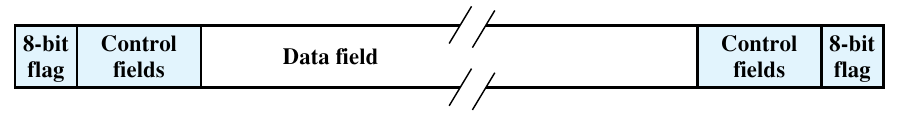
\includegraphics[width=0.7\linewidth]{gambar/fig:06.02}
	\caption{Synchronous Frame Format}
	\label{fig:06.02}
\end{figure}


\section{Frequency-Division Multiplexing}

\section{Synchronous Time-Division Multiplexing}

\section{Cable Modem}

%%%%%%%%%%%%%%%%%%%%%%%%%%%%%%%%%%%%%%%%%%%%%%%%%%%
\section{Asymmetric Digital Subscriber Line (ADSL)}

Dalam mengimplementasikan dan menyebarkan high-speed wide area public digital network, bagian yang paling menantang adalah link antara subscriber dan network: digital subscriber line. Dengan jutaan potensial endpoint di seluruh dunia, prospek menginstal kabel baru untuk masing-masing pelanggan baru adalah hal yang menakutkan. Sebagai gantinya, network designer


\section{xDSL}